\chapter{Introduction}

\section{Motivation}

Carbonaceous nanoparticles, such as Carbon Black (CB) and soot, are widely encountered in nature and engineering. Every year, nearly 9.5 megatons of soot are emitted into the atmosphere from anthropogenic activities and natural sources such as wildfires and volcanoes~\citep{myhre2014anthropogenic}. The wide light absorption range of soot reduces the albedo of snow-covered areas and alters the radiative forcing balance in the atmosphere, making soot the third strongest contributor to climate change after methane and carbon dioxide~\citep{myhre2014anthropogenic}. Exposure to combustion-generated soot can also promote respiratory and cardiovascular diseases~\citep{world2013health}. Strict regulations thus target combustion engines to limit environmental and health risks from soot formation~\citep{integrated2019}. Accurate and affordable models are essential for predicting soot composition and morphology in combustion devices and for reducing emissions in engines. They can also provide better understanding of soot optical properties, which are major indicators of soot's environmental effects.

%Carbonaceous nanoparticles, such as Carbon Black (CB) and soot, are widely encountered in nature and engineering. Every year, nearly 9.5 megatons of soot is emitted into the atmosphere from anthropogenic activities and natrual sources such as wildfires and volcanoes~\citep{myhre2014anthropogenic}. The wide light absorption range of soot reduces the albedo of snow-covered area and alters the radiative forcing balance in the atmosphere making soot the third strongest contributor to climate change after methane and carbon dioxide~\citep{myhre2014anthropogenic}. Also, exposure to combustion-generated soot could promote respiratory and cardiovascular diseases~\citep{world2013health}. So, strict regulations are targeting combustion engines to limit environmental and health risks from soot formation~\citep{integrated2019}. Accurate and affordable models are essential for the prediction of soot composition and morphology in combustion devices and the reduction of emissions in engines. They can also provide better understanding of soot optical properties that are major indicator of soot environmental effects.

On the other hand, CB with a similar synthesis process and structure to soot but higher elemental carbon to hydrogen ratio ($>$97\%)~\citep{watson2001carbon} is commercially produced and sold on a large scale. In fact, CB is the largest industrially produced nanomaterial by value and volume ($\sim$15 megatons per year with a value of $\sim$\$17B) with applications as a reinforcing agent in rubber and tire industries~\citep{international2016carbon}, and as a conductive additive in lithium-ion batteries~\citep{Palomares2010}. CB is primarily manufactured by the furnace process in which about 50\% of heavy fuel oil is partially combusted to convert the rest into CB~\citep{pratsinis2011history}. This process suffers from low mass yield and excessive emissions, generating 4 tons of CO$_2$ per ton of product on average~\citep{bansal1993carbon}. Plasma reactors are emerging as an alternative production method with distinct advantages over flame-based methods: they can achieve 100\% carbon yields with no direct CO$_2$ emissions or other pollutants~\citep{cho2004conversion}, and the energy required for pyrolysis is supplied by an electric arc that does not depend on the feedstock composition. Controlling CB properties such as its specific surface area (or primary particle diameter), hard agglomerate size (or gyration diameter of agglomerates with primary particles connected by strong chemical bonds), and composition (or particle carbon-to-hydrogen ratio) is important to make the process economical and to achieve specific grades of CB for different target applications. However, this is challenging because of the complexity of CB formation and mass growth processes, their coupling with gas-phase chemistry, and dependence on local temperature and pressure. Accurate process design and optimization tools are thus required to inform manufacturers' decisions for production of CB with desired grades~\citep{park2005influence}.

%On the other hand, CB with a similar synthesis process and structure to soot but higher elemental carbon to hydrogen ratio ($>$97\%)~\citep{watson2001carbon} is commercially produced and sold in large scales. In fact, CB is the largest industrially produced nanomaterial by value and volume ($\sim$15 megatons per year with a value of $\sim$\$17B) with applications as a reinforcing agent in rubber and tire industries~\citep{international2016carbon}, and conductive additive in lithium-ion batteries~\citep{Palomares2010}. CB is primarily manufactured by the furnace process in which about 50\% of heavy fuel oil is partially combusted to convert the rest of it into CB~\citep{pratsinis2011history}. This process suffers from low mass yield and excessive emissions, generating 4 tons of CO$_2$ per each ton of product on average~\citep{bansal1993carbon}. Plasma reactor is an emerging alternative production method with distinct advantages over flame-based methods: They can achieve 100\% carbon yields with no direct CO$_2$ emission or other pollutants~\citep{cho2004conversion}, and the energy required for pyrolysis is supplied by an electric arc that does not depend on the feedstock composition. Controlling CB properties such as its specific surface area (or primary particle diameter), hard agglomerate size (or gyration diameter of agglomerates with primary particles connected to each other by strong chemical bonds), and composition (or particle carbon-to-hydrogen ratio) is important to make the process economical and to achieve specific grades of CB for different target applications. However, this is a challenging task because of the complexity of CB formation and mass growth processes, its coupling with gas phase chemistry, and dependence on local temperature and pressure. This requires accurate process design and optimization tools to inform manufacturers' decisions for production of CB with desired grades~\citep{park2005influence}.
 
The term \textit{soot} usually refers to unwanted particulate matter formed during incomplete combustion of carbon-containing materials ranging from jet and diesel fuel to wood, heavy oil, and plastics, with variable organic content and a wide range of C/H ratios~\citep{watson2001carbon}. However, this research focuses on soot particles generated under controlled laboratory conditions from fuels with known compositions. Mature soot formed in methane and ethylene premixed flames can reach 95\% elemental C/H ratio~\citep{russo2015dehydrogenation}, which is close to CB composition. The comparison of transmission electron microscopy (TEM) images of industrially produced CB~\citep{singh2018nanostructure} with soot sampled from diesel fuel~\citep{vander2007hrtem, lapuerta2017morphological}, shown in Fig.~\ref{fig:sootCBHRTEM}, indicates similarity in their morphology and structure. Hereafter, soot will be used to collectively refer to carbonaceous nanoparticles produced in flames or reactors during combustion or pyrolysis processes. 
 
%The term \textit{"soot}" usually refers to the unwanted particulate matter formed during incomplete combustion of any carbon-containing material from jet and diesel fuel to wood, heavy oil, and plastics with variable organic content and a large variation in C/H ratio~\citep{watson2001carbon}, but this research focuses on soot particles generated under controlled laboratory conditions from fuels with known compositions. The mature soot formed in methane and ethylene premixed flame can reach 95\% elemental C/H ratio~\cite{russo2015dehydrogenation}, which is close to CB composition. The comparison of transmission electron microscopy (TEM) images of industrially produced CB~\citep{singh2018nanostructure} with soot sampled from diesel fuel~\citep{vander2007hrtem, lapuerta2017morphological} shown in Fig.\ref{fig:sootCBHRTEM} indicates similarity of their morphology and structure. Hereafter, soot will be used to collectively refer to carbonaceous nanoparticles produced in flame/reactor during combustion/pyrolysis processes.

\begin{figure}[!t]
	\centering
	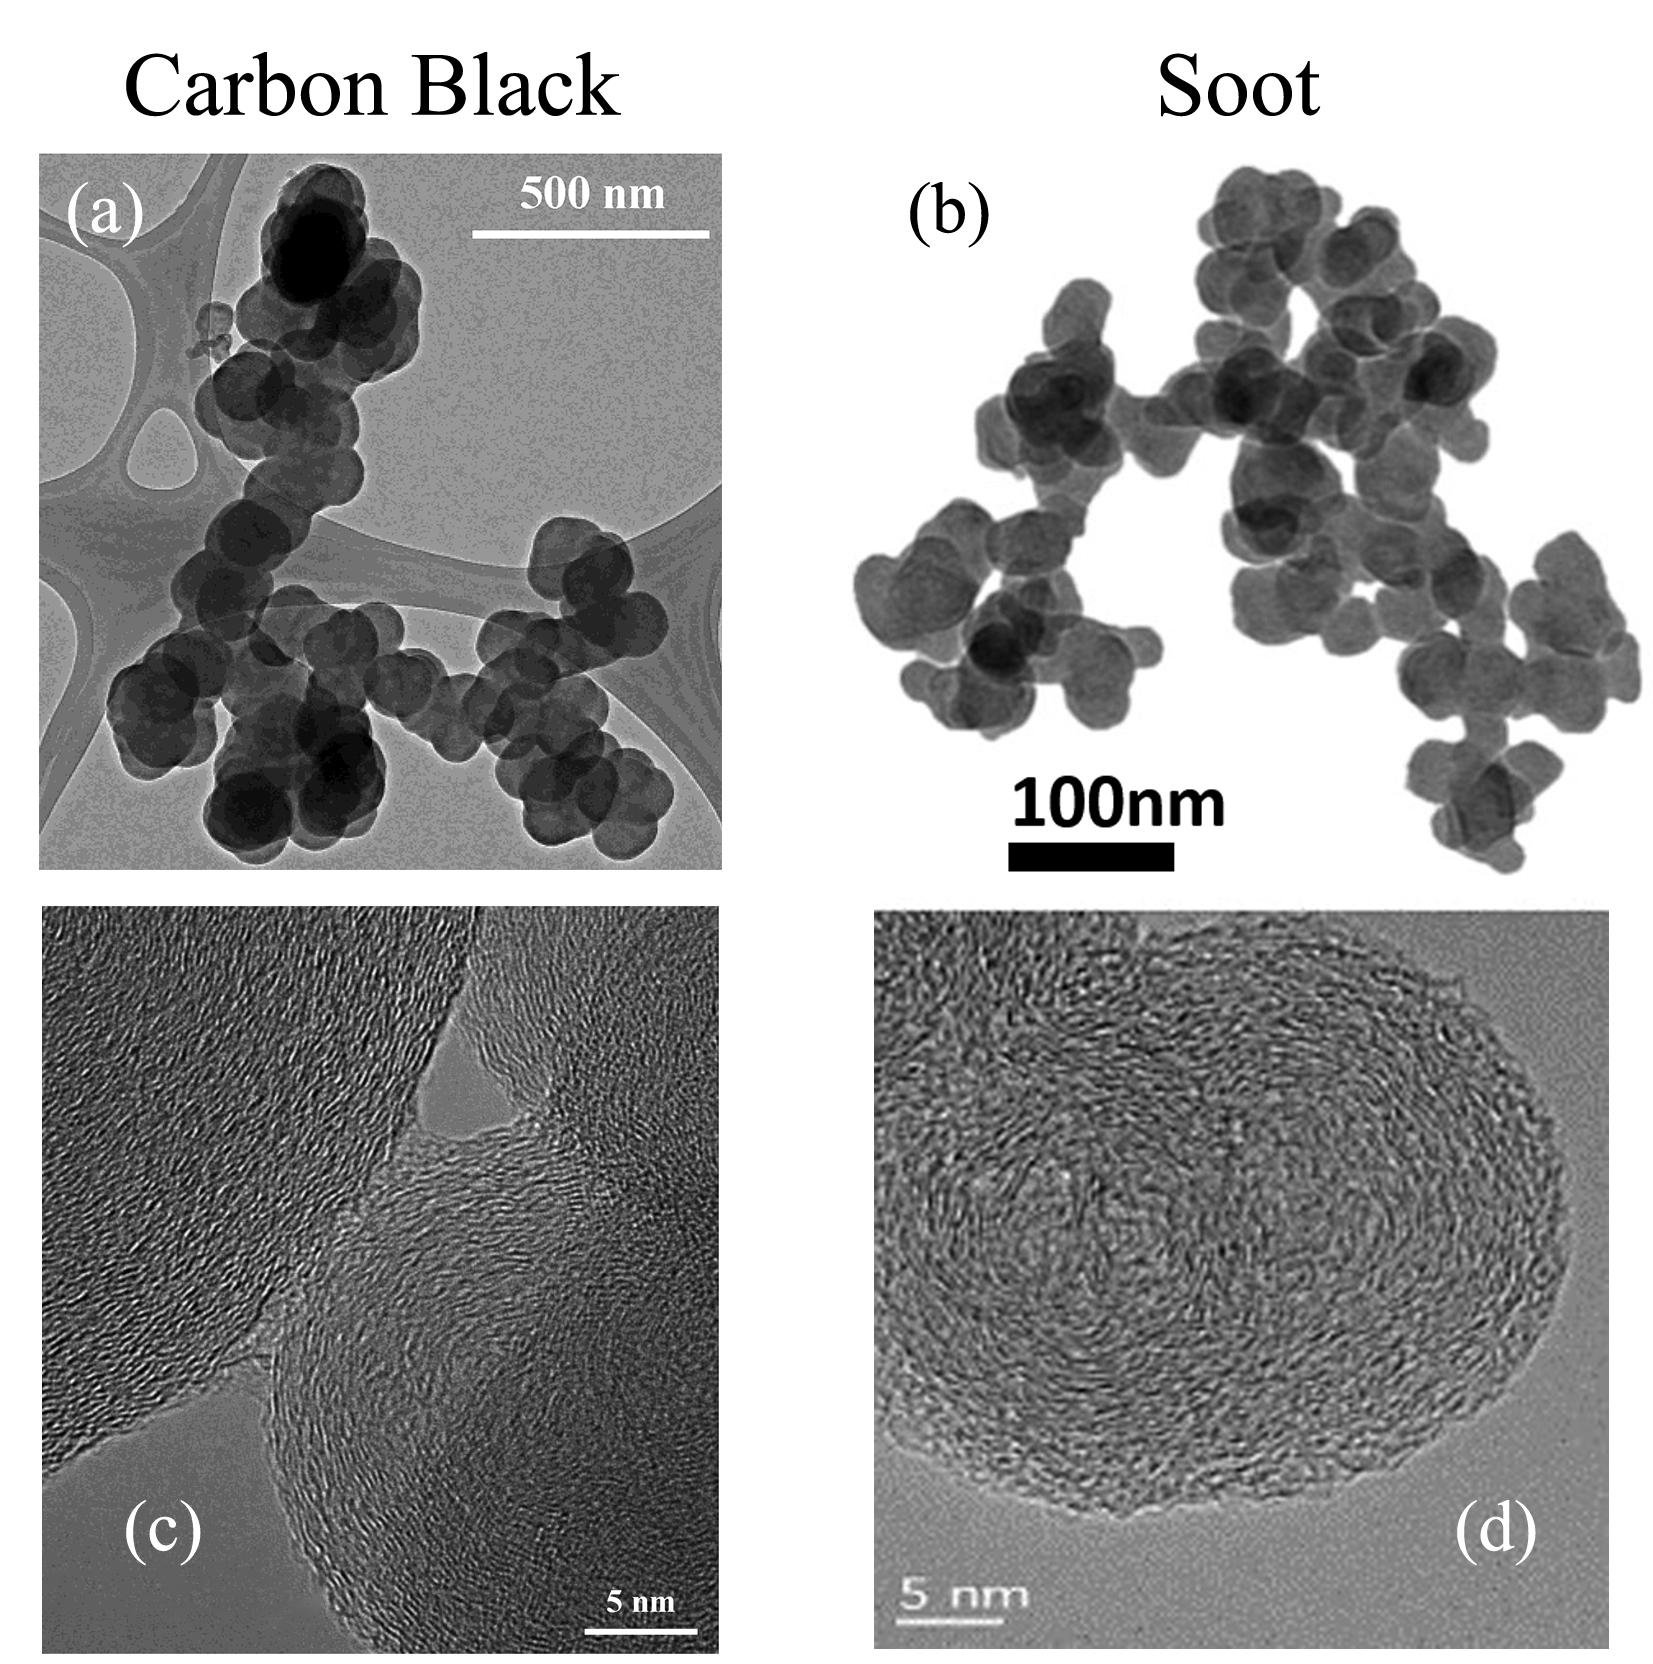
\includegraphics[width=0.6\textwidth, ]{Figures/Introduction/soot_CB_HRTEM.jpg}
	\caption[The TEM images of Carbon black (a \& c) and soot (b \& d)
	that shows soot and CB has similar morphology and nanostructure]{The TEM images of Carbon black (a \& c)~\citep{singh2018nanostructure} and soot (b \& d)~\citep{vander2007hrtem, lapuerta2017morphological}
	 that shows soot and CB has similar morphology and nanostructure.}
 	\label{fig:sootCBHRTEM}
\end{figure} 



\section{Background}
\subsection{Soot inception and surface growth}
Soot formation involves concurrent processes with different time and length scales, starting from the breakdown of hydrocarbon molecules to formation of intermediate species and radicals that transition into soot particles and grow via heterogeneous surface reactions as well as coagulation~\citep{d2009combustion}. TEM analysis of soot sampled from flames~\citep{lapuerta2017morphological}, reactors~\citep{ono2017experimental}, and engines~\citep{wei2020morphology} with different fuels and process conditions revealed a common fractal-like morphology, often characterized as agglomerates of primary particles. High-resolution transmission electron microscopy (HRTEM) of soot primary particles showed clusters of precondensed polycyclic aromatic hydrocarbons (PAH)~\citep{alfe2009structure}, pointing to PAHs as main soot precursors. This hypothesis was also supported by the thermodynamic stability of PAHs, enabling them to resist dissociation at high flame temperatures~\citep{stein1985high}.

However, the transition of PAHs (soot precursors) to incipient soot, known as \textit{soot inception}, has not been well understood at the level of pathways and elementary reactions~\cite{Wang2011}, primarily due to uncertainties in PAH (precursor) chemistry. The formation of carbonaceous particles is kinetically controlled and is known to be an entropy-driven process~\cite{Wang2011}. \citet{Wang2011} used the pyrolysis of propane at 1600~K to highlight how the thermodynamics of soot formation differ from those of inorganic nanomaterial synthesis. As shown in Fig.~\ref{fig:gibbschange}, acetylene formation is highly endothermic, but it is accompanied by a drastic increase in entropy due to hydrogen release, resulting in an overall decrease in Gibbs free energy, which explains why acetylene (C$_2$H$_2$) is the dominant hydrocarbon species. The growth of PAHs from acetylene does not involve a significant enthalpy release or entropy increase, so the pathway is driven by a gradual reduction in Gibbs free energy. As a result, the kinetics of PAH growth into subsequent soot particles can be highly reversible and therefore sensitive to local temperature, pressure, and intermediate species concentrations.

\begin{figure}[!t]
	\centering
	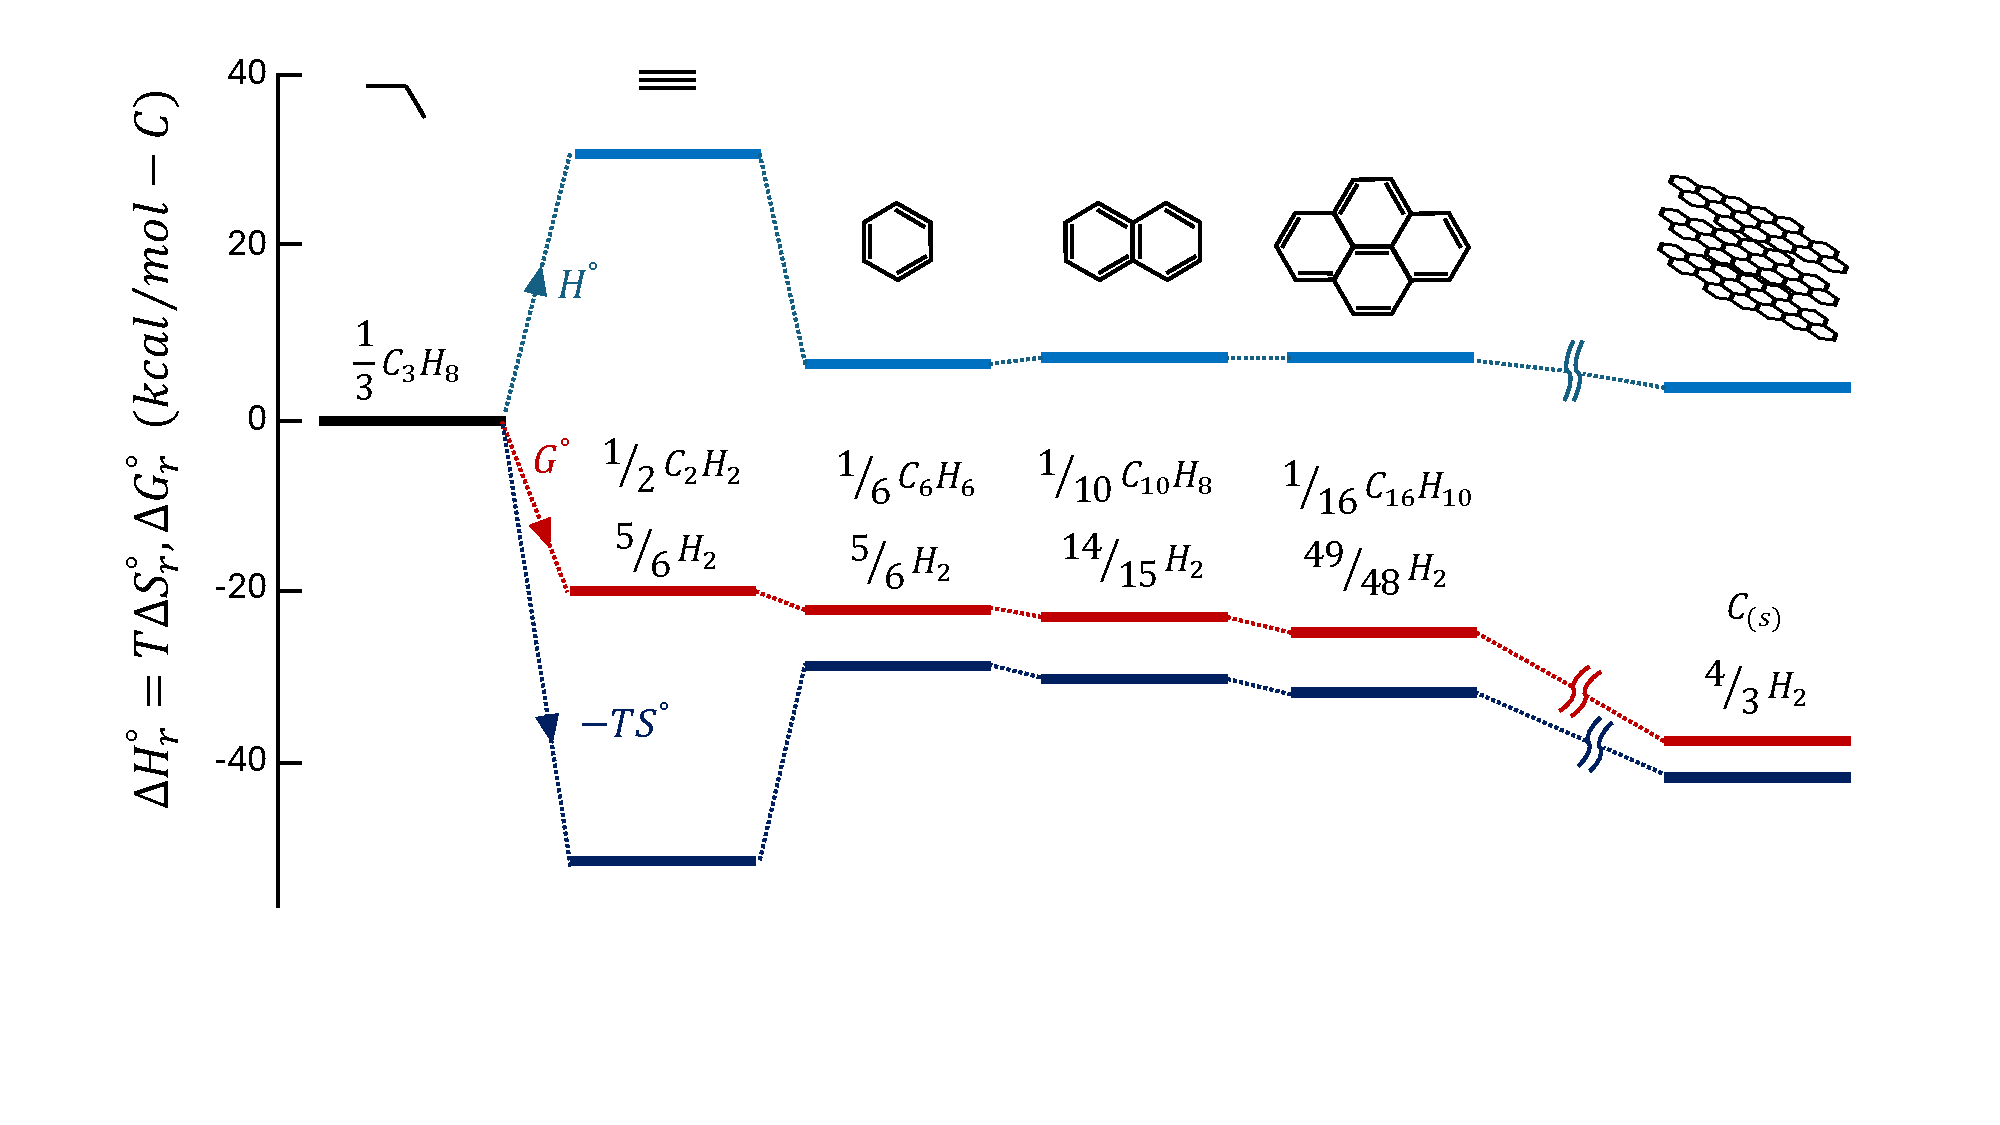
\includegraphics[width=0.9\textwidth, ]{Figures/Introduction/gibbs_propane.pdf}
	\caption[Standard enthalpy (${\Delta H}$) and entropy (${T\Delta S}$) contributions to Gibbs function of reaction $\mathrm{\Delta G}$ at 1600 K for carbon formation from propane]{Standard enthalpy (${\Delta H}$) and entropy (${T\Delta S}$) contributions to Gibbs function of reaction $\mathrm{\Delta G}$ at 1600 K for carbon formation from propane (reprinted from Ref.~\citep{Wang2011})}
	\label{fig:gibbschange}
\end{figure} 

%However, the transition of PAHs (soot precursors) to incipient soot, known as \textit{soot inception} has not been well understood at the level of pathways and elementary reactions~\cite{Wang2011} primarily due to uncertainties in PAH (precursor) chemistry. The formation of carbonaceous particles is kinetically controlled and known to be an entropy-driven process~\cite{Wang2011}. \citet{Wang2011} uses the pyrolysis of propane at 1600 K to highlight how thermodynamics of soot formation is distinct from synthesis of inorganic nanomaterials. As shown in Fig.~\ref{fig:gibbschange}, acetylene is highly endothermic, but it is accompanied with drastic increase in entropy due to hydrogen release resulting in overall decrease of Gibbs free energy, which explains acetylene ($\mathrm{C_2H_2}$) being the dominant hydrocarbon species. The growth of PAHs from acetylene does not undergo a significant enthalpy release or entropy increase, so the path is driven by a gradual reduction in Gibbs free energy. As a result, the kinetics of PAH growth into subsequent soot particles can be highly reversible hence sensitive to local temperature, pressure and intermediate species concentration.

The growth of PAHs beyond the first ring (benzene) is predominantly driven by the so-called hydrogen abstraction carbon (acetylene) addition (HACA) mechanism~\citep{frenklach2002reaction}, where a hydrogen radical abstracts a hydrogen atom at the edge of a PAH, providing a reactive site for acetylene addition. The kinetic reversibility of HACA opens the door for competing pathways such as chain reactions of resonance-stabilized radicals (RSR). Propargyl is a prominent example of these radicals, whose combination is known as a major contributor to benzene formation~\citep{fahr1989reactions}. Building on this hypothesis, \citet{johansson2018resonance} proposed a radical-driven growth mechanism by addition of vinyl ($\mathrm{C_2H_3}$) starting from cyclopentadienyl ($\mathrm{C_5H_5}$) to larger hydrocarbon radicals that can survive long enough at high temperatures to react with other radicals, PAHs, and unsaturated aliphatic species through radical chain reactions. However, low concentrations of these radicals limit the growth rate through RSR pathways~\citep{frenklach2020mechanism}. Moreover, some intermediate steps for radical regeneration, such as formation of vinylcyclopentadienyl, were shown to be kinetically unfavorable~\citep{frenklach2020mechanism} compared to HACA. Regardless of their mechanistic details, these sequential growth mechanisms, termed \textit{chemical growth}, cannot account for rapid soot formation~\citep{frenklach2002reaction} and its nanostructure~\citep{frenklach1988comment}.

%The growth of PAHs beyond first ring (benzene) is predominantly driven by so-called hydrogen abstraction carbon (acetylene) addition (HACA) mechanism~\citep{frenklach2002reaction} where a hydrogen radical abstracts an hydrogen atom at the edge of PAH, providing a reactive site for acetylene addition. The kinetic reversibility of HACA opens the door for competing pathways such as chain reactions of resonance-stabilized radical (RSR). Propargyl is a prominent example of these radicals, whose combination is known as a major contributor to benzene formation~\citep{fahr1989reactions}. Built on this hypothesis, \citet{johansson2018resonance} proposed a radical-driven growth mechanism by addition of vinyl ($\mathrm{C_2H_3}$) starting from cyclopentadienyl ($\mathrm{C_5H_5}$) to larger hydrocarbon radicals that can survive long enough in high temperatures to react with other radicals, PAHs and unsaturated aliphatic species, through radical chain reactions. However, low concentrations of these radicals limit the growth rate through RSR pathways~\citep{frenklach2020mechanism}. Moreover, some of the intermediate steps for radical regeneration such as formation of vinylcyclopentadienyl were shown to be kinetically unfavorable~\citep{frenklach2020mechanism} compared to HACA. Regardless of their mechanistics, these sequential growth mechanisms, termed as \textit{chemical growth} cannot account for rapid soot formation~\citep{frenklach2002reaction} and its nanostructure~\citep{frenklach1988comment}.

There is abundant but mostly indirect experimental and computational evidence pointing to an alternative collision-based mechanism for soot inception. HRTEM images of nascent and mature soot shows disordered PAH clusters highlighting the role of PAH collisions. The bimodality of particle size distribution (PSD) of nascent soot particles in premixed flames~\citep{zhao2003measurement} indicates that the kinetics of inception is second order in precursor concentration~\citep{abid2009quantitative}. The time-of-flight mass spectrometry (TOFMS) experiments in a 13 kPa acetylene-oxygen flame showed a series of peaks with a periodicity of 500 amu~\citep{happold2009soot}. 

It is not clear how PAH clusters form and what forces allow binding to occur and resist dissociation at flame temperatures (T$\ge$1600~K). \citet{frenklach2002reaction} described clustering of PAHs as an irreversible process where two PAHs collide and stick upon collision, forming dimers held together by van der Waals (vdW) forces. \citet{herdman2008intermolecular} found that the binding energy of PAH dimers due to dispersive and electrostatic forces increases linearly with molecular mass and reaches the limit of graphite exfoliation energy. However, the entropy barrier of dimerization increases with PAH size, making it unfavorable under equilibrium conditions. Thus, PAHs as large as circumcoronene (C$_{54}$H$_{18}$) can only form dimers that survive flame temperatures~\citep{Wang2011}. However, the concentrations of large PAHs are too low to account for the observed number density of soot particles in flames~\citep{totton2012quantitative}.

%It is not clear how PAH clusters form and what forces allow the binding occur and resist dissociation at flames temperatures (T$\ge$1600 K). \citet{frenklach2002reaction} described clustering of PAHs as an irreversible process where two PAHs collide and stick upon collision forming dimers held together by Van der Waals (vdW). \citet{herdman2008intermolecular} found that the binding energy of PAHs dimers due to dispersive and electorstatic forces increases linearly with molecular mass and reaches the limit of exfoliation energy for graphite. However, the entropy barrier of dimerization increases with PAH size making them unfavorable under equilibrium conditions. So, PAHs as large as circumcoronene ($\mathrm{C_{54}H_{18}}$) can only form dimer to survive flame temperatures~\citep{Wang2011}. However, the concentration of large PAHs are too low to account for the observed number density of soot particles in flames~\citep{totton2012quantitative}. 

There is also the possibility of PAH clustering governed by non-equilibrium kinetics. PAH molecules can form rovibrationally excited dimers with a long enough lifetime~\cite{wong2009molecular} to react with H atoms, forming covalent bonds. Another possibility is that these clusters are joined by aliphatic linkages. Micro-FT-IR spectroscopy analysis by \citet{cain2011evidence} showed that the ratio of aliphatic-to-aromatic C–H bonds can exceed unity at flame temperatures. Using these findings, they suggested that aliphatic components in the form of alkyl and alkenyl groups can covalently bind to aromatic units in soot particles. Although such a mechanism is viable near the flame region, it cannot explain persistent soot inception in the post-flame zone~\citep{zhao2005particle}, where the H atom concentration is too low to initiate H abstraction reactions that produce those radicals.

%There is also the possibility of PAH clustering governed by non-equilibrium kinetics. PAH molecules can form rovibrationally excited dimer with long enough life-time~\cite{wong2009molecular} to react with H atoms forming covalent bonds. There is another possibility for these clusters to be joined by aliphatic linkages. Micro-FT-IR spectroscopy analysis by \citet{cain2011evidence} showed the ratio of aliphatic-to-aromatic C–H bonds can exceed unity at the flame temperature. Using these findings, they suggested that the aliphatic components in the form of alkyl and alkenyl can covalently bound to aromatic units in soot particles. Although such a mechanism is viable near the flame region, it cannot explain persistent soot inception in the post-flame zone~\citep{zhao2005particle} where the H atom concentration is too low to initiate H abstraction reactions that produce those radicals.


There are other complicating factors that hinder the fundamental understanding of soot inception, such as the lack of a decisive criterion to distinguish gaseous molecules from particles~\citep{d2009combustion}, and the overlap of inception with surface growth and agglomeration~\citep{martin2022soot}. Measurement techniques have limited capability for soot detection due to the short time and length scales of soot inception and surface growth, ranging from picoseconds to milliseconds and micrometers to millimeters~\citep{violi2005relative}. Fig.~\ref{fig:sootscales} demonstrates the length and time scales relevant to different stages of soot formation from PAH precursors to incipient, nascent, and mature soot in flames. Moreover, data collected from measurements might not be true representatives of soot formed at the probed location in the studied process. For example, intrusive diagnostic methods based on thermophoresis or dilution have a sampling probe that can perturb flow dynamics or alter the structure and composition of soot~\citep{kholghy2017comparison}. Non-intrusive techniques such as optical methods also rely on assumptions about the light absorption and scattering of soot~\citep{shaddix1996laser} and its morphology~\citep{doner2017impact}.

%There are other complicating factors that hinders the fundamental understanding of soot inception such as lack of a decisive criterion to distinguish gaseous molecules from particles~\citep{d2009combustion}, and the overlap of inception with surface growth and agglomeration~\cite{martin2022soot}. Measurement techniques have limited capability in soot detection due to short time and length scales of soot inception and surface growth ranging from pico- to milliseconds and micro- to millimeter~\citep{violi2005relative}. Fig.~\ref{fig:sootscales} demonstrates the length and time scales relevant to different stages of soot formation from PAH precursors to incipient, nascent and mature soot in flames. Moreover, the collected data from measurements might not be true representatives of soot formed at the probed location of the studied process. For example, intrusive diagnostic methods based on thermophoresis or dilution have a sampling probe that can perturb flow dynamics or alter structure and composition of soot~\cite{kholghy2017comparison}. Non-intrusive techniques such as optical methods also rely on assumptions about light absorption and scattering of soot~\citep{shaddix1996laser} and its morphology~\citep{doner2017impact}.

Despite the gaps in fundamental understanding of soot formation and limitations of diagnostic methods, models have been developed to describe soot inception and growth. These models have been formulated as a set of clear pathways that explain soot inception based on collisions of PAH molecules. They must be consistent with current knowledge of soot inception, feasible to couple with chemistry and particle dynamics models, and able to predict soot mass, PSD, and morphology observed in flames and reactors.

%Despite the gaps in fundamental understanding of soot formation and limitations of diagnostics methods, models have been developed describe the soot inception and growth. These models have been formulated as a set of clear pathways that explain soot inception based on collisions of PAH molecules. They have to be consistent with current knowledge of soot inception, feasible to be coupled with chemistry and particle dynamics models, and able to predict soot mass, PSD and morphology observed in flames and reactors.

The classic description of soot inception relies on PAH dimerization, where collision of two PAH molecules (monomers in this context) forms a dimer held together by van der Waals forces~\citep{frenklach1991detailed}. The dimerization is modeled as an irreversible process with an efficiency that accounts for the reversibility or dissociation of dimers. The theory postulates that PAH growth continues by sequential addition of a monomer (PAH molecule), forming stacks of dimers, trimers, tetramers, and so on to reach a certain mass threshold that marks the emergence of incipient soot~\citep{frenklach1991detailed}, but for practical purposes, a dimer is usually considered as incipient soot. Here, we call this model \textit{Irreversible Dimerization}. Irreversible Dimerization has been used to predict soot formation in burner-stabilized premixed~\citep{salenbauch2015modeling, desgroux2017comparative}, counterflow diffusion~\citep{wang2015soot, xu2021experimental}, and coflow diffusion flames~\citep{kholghy2016core, veshkini2016understanding}. A collision efficiency factor ranging between $10^{-6}$ and 1 is also employed to adjust the inception flux and PAH adsorption rates to achieve the desired soot mass and size distribution. PAHs of moderate sizes, such as pyrene (4 rings) to coronene (7 rings), have been considered as the starting point of inception due to their thermodynamic instability, which justifies the irreversibility at high temperatures~\citep{frenklach1991detailed}. However, theoretical calculations~\citep{miller1985calculations} and experiments~\citep{sabbah2010exploring} indicate that PAH dimerization is highly reversible under flame conditions.

%The classic description of soot inception relies on PAH dimerization where collision of two PAH molecules (monomers in this context) forms a dimer held together by Van der Wales forces~\citep{frenklach1991detailed}. The dimerization is a irreversible process with an efficiency that accounts for the reversibility or dissociation of dimers. The theory postulates that PAH growth continues by sequential addition of a monomer (PAH molecule) forming stacks of dimers, trimers, tetramers and so on to reach a certain mass threshold that marks the emergence of incipient soot~\citep{frenklach1991detailed}, but for practical purposes, a dimer is usually considered as an incipient soot. Here, we call this model \textit{Irreversible Dimerization}. Irreversible Dimerization has been used to predict soot formation in burner-stabilized premixed~\citep{salenbauch2015modeling, desgroux2017comparative}, counterflow diffusion flames~\citep{wang2015soot, xu2021experimental}, coflow diffusion flames~\citep{kholghy2016core, veshkini2016understanding}. A collision efficiency factor ranging between $10^{-6}$ to 1 is also employed to adjust the inception flux and PAH adsorption rates to achieve desired soot mass and size distribution. PAHs of moderate sizes such as pyrene (4 rings) to coronene (7 rings) have been considered as the starting point of inception due to their thermodynamic instability that justifies the irreversibility at high temperatures~\citep{frenklach1991detailed}. However, the theoretical calculations~\citep{miller1985calculations} and experiments~\citep{sabbah2010exploring} indicated that PAH dimerization is highly reversible in flame conditions.



% Fringe analysis from Jacob's paper 

%  “chemical similarity” hypothesis in "Unified Kinetic Model of Soot Formation in the Pyrolysis and Oxidation of Aliphatic and Aromatic Hydrocarbons in Shock Waves"

% Maybe use discussion in nucleation flame paper to argue for a collision-based proxy inception model 

%  are limited by possible ~\citep{buesser2012design} due to coupling with gas chemistry~\cite{Wang2011}, dependence on local temperature~\citep{gleason2018effect} and pressure~\cite{gleason2021pahs}. It has also been challenging to pinpoint the start of inception because of its short time scales in the order $10^{-9}$ s~\citep{buesser2012design}, the lack of a decisive criterion to distinguish molecules from particles~\citep{d2009combustion}, and the overlap of inception with particle growth and agglomeration~\cite{martin2022soot}. Despite these limitations and challenges, our knowledge about soot formation has significantly increased thanks to advances in diagnostics methods and reaction mechanism development. 

\begin{figure}[!t]
	\centering
	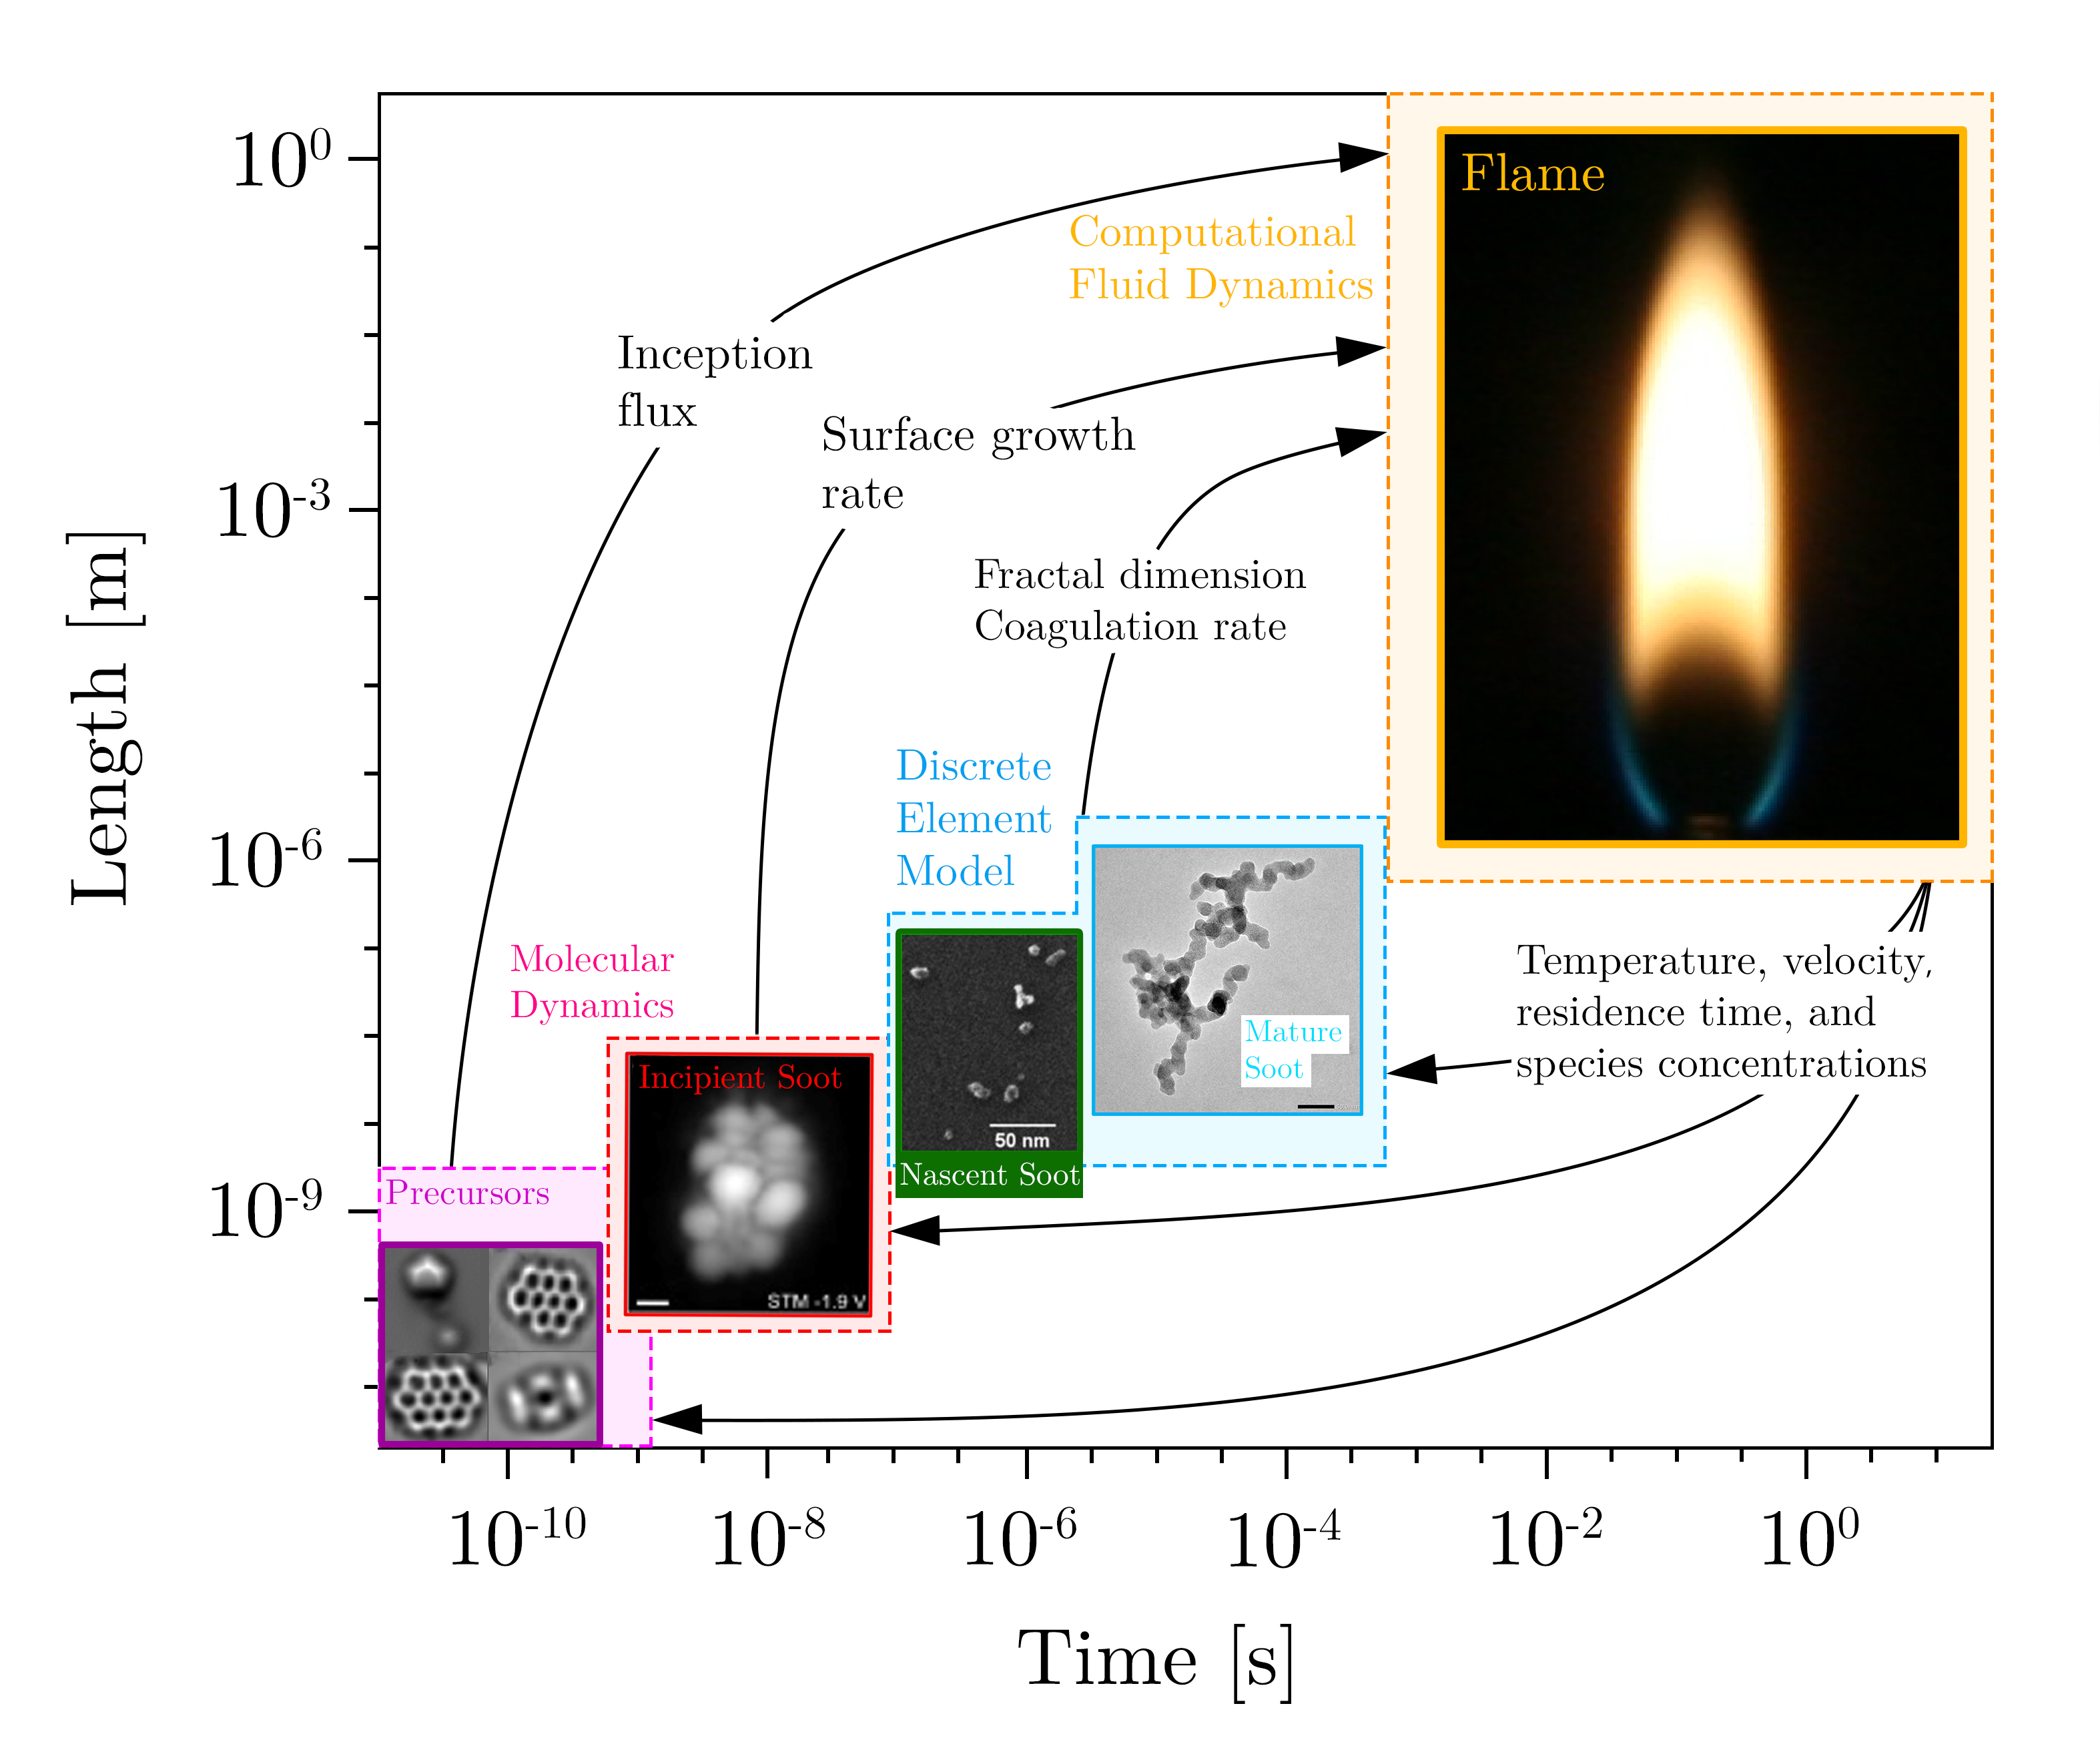
\includegraphics[width=0.8\textwidth, ]{Figures/Introduction/tlscales.jpg}
	\caption{The range of time and length scales of the processes involved in soot formation from molecular reactions to particle-fluid interaction in flames}
	\label{fig:sootscales}
\end{figure}



%There is compelling evidence that highlights the role of Polycyclic Aromatic Hydrocarbons (PAH) as the main soot precursors. They are thermodynamically stable enough to withstand dissociation at high flame temperatures~\citep{stein1985high} and observed in stacked layers in High Resolution Transmission Electron Microscope (HRTEM) images of soot primary particles~\citep{Oberlin1984}. 
%\hl{[placeholder for literature review on the role of diradicals and resonantly stabilized radicals in soot inception]}

%But, the two important questions need to be answered: (1) which PAHs contribute most to the inception, and (2) what pathways best describe PAH to incipient soot transition. Purely chemical growth mechanisms are shown to underpredict inception rates and particle size~\citep{frenklach2002reaction}. The bimodality of particle size distribution in premixed flames~\citep{camacho2015mobility} suggests a mechanism second order with respect to the monomer~\citep{Wang2011}. To satisfy these requirements, a collision-based inception was proposed where irreversible polymerization form PAH clusters held together by Van der Wales forces. The theory postulates that PAH growth continues to reach a certain mass threshold that marks emergence of solid particles, but for practical purposes, a dimer is usually considered as incipient soot. 

%In this model, hereafter referred to as \textbf{Irreversible Dimerization}, the collision of two PAH molecules is assumed to form a dimer
% that gains mass via two growth mechanisms: (i) hydrogen-abstraction-carbon-addition (HACA) that assumes soot surface to consist of hydrogenated sites with predefined density that can lose hydrogen and react with acetylene (ii) collision of PAH molecules/clusters with soot particles leading to chemisorption. 
 

The inception flux of irreversible dimerization is determined from PAH collisions, which is proportional to $\sqrt{T}$, so new particles can form at low temperatures (even below 500~K)~\citep{naseri2022simulating}, despite experimental evidence for termination of inception below 1200~K~\citep{sanchez2012polycyclic, cho2016synthesis}. Moreover, the arbitrary selection of efficiency factors, which alters the distribution of mass between inception and surface growth, can significantly change soot mass, PSD, and morphology~\citep{saffaripour2014experimental}.  A two-step irreversible model, referred to here as \textit{Dimer Coalescence}, was proposed by Blanquart and Pitsch~\citep{blanquart2009analyzing}. In this model, PAH molecules collide with each other to form dimers, which represent an intermediate state between gas-phase PAHs and solid soot particles. These dimers can either undergo self-coalescence to form incipient soot particles or adsorb onto existing soot surfaces, contributing to their surface growth.

% \citet{miller1991kinetics} used the equilibrium constant for PAH dimerization to calculate the net dimerization rate and demonstrated that collisions of PAHs larger than circumovalene ($\sim$800~amu) could last long enough to grow into incipient soot. However, the concentration of PAHs drops rapidly with size~\citep{Wang2011}.


%The inception flux of irreversible dimerization is determined from collision of PAHs, which is proportional to $\sqrt{T}$, so new particles can be formed at low temperatures (even less than 500 K)~\citep{naseri2022simulating} despite experimental evidence for termination of inception below 1200 K~\citep{sanchez2012polycyclic, cho2016synthesis}. Moreover, the arbitrary selection of efficiency factors alters the distribution of mass between inception of surface growth could significantly change soot mass, PSD, and morphology~\citep{saffaripour2014experimental}. \citet{miller1991kinetics} used equilibrium constant for PAH dimerization to calculate the net dimerization rate and demonstrated that the collision of PAHs larger than circumovalene ($\sim$800 amu) could last long enough grow into incipient soot. However, the concentration of PAHs drops rapidly with size~\citep{Wang2011}.


% The entropy barrier of dimerization is significant for larger PAHs~\citep{giordana2011theoretical}.  


\citet{eaves2015importance} relaxed the irreversibility assumption and developed a reversible clustering model to simulate inception using an array of PAHs from naphthalene to benzo-pyrene. Building on that work, \citet{kholghy2019role} emphasized the necessity of chemical bond formation after physical PAH clustering for accurate prediction of volume fraction, primary particle diameter, and PSD in ethylene coflow diffusion flames. Later, \citet{kholghy2018reactive} proposed the \textit{"Reactive Dimerization"} model, which starts with reversible collision of PAHs leading to physically bonded dimers held by vdW forces. Physical dimers can then be graphitized to form chemically bonded dimers that serve as soot nuclei and grow via surface reactions. \citet{kholghy2018reactive} also performed a systematic analysis of the contribution of different PAHs and concluded that one- and two-ring aromatics account for almost all of the inception flux in the so-called \textit{"sooting flame"}~\citep{desgroux2017comparative}. However, \citet{frenklach2020mechanism} pointed out that an inception model initiated with a highly reversible step similar to Reactive Dimerization~\citep{kholghy2018reactive} cannot produce sufficient particle flux to match measurements from the benchmark burner-stabilized stagnation flame~\citep{abid2009quantitative}. Instead, they proposed a HACA-driven mechanism where addition of a monomer molecule to its radical, activated by hydrogen abstraction, forms a stable dimer via E-Bridge bond formation, and this sequential process continues to form trimers, tetramers, and larger PAH clusters.

%\citet{eaves2015importance} relaxed the irreversibility assumption, and developed a reversible clustering model to simulate inception using an array of PAHs from naphthalene to benzo-pyrene. Building on that work, \citet{kholghy2019role} emphasized on the necessity of chemical bond formation after physical PAH clustering for accurate prediction of volume fraction, primary particle diameter and PSD in ethylene coflow diffusion flames. Later, \citet{kholghy2018reactive} proposed the \textit{"Reactive Dimerization"} model which starts with reversible collision of PAHs leading to physically-bonded dimers held with vdW forces. Physical dimers can be graphitized and form chemically-bonded dimers that serve as soot nuclei grow via surface reactions. \citet{kholghy2018reactive} also performed a systematic analysis on the contribution of different PAHs, and concluded that one- and two-ring aromatics account for almost all of inception flux in the so-called \textit{"sooting flame"}~\citep{desgroux2017comparative}. However, \citet{frenklach2020mechanism} pointed out that an inception model that initiated with a highly reversible step similar to Reactive Dimerization~\citep{kholghy2018reactive} cannot produce sufficient flux of particles to match measurements of the benchmark burner-stabilized stagnation flame~\citep{abid2009quantitative}. Instead, they proposed a HACA-driven mechanism where addition of monomer molecule to its radical activated by hydrogen abstraction for a stable dimer via an E-Bridge bond formation, and this sequential process continues to form trimers, tetramers, and larger PAH clusters.

The gas-phase chemistry of aromatics can be extended to account for chemical growth of incipient soot via surface reactions~\citep{frenklach2002reaction}. This hypothesis, known as “chemical similarity,” postulates that the reactions occurring on the soot surface are similar to those involving large PAH molecules in the gas phase. It also provides a means to describe the rates of surface growth and particle oxidation in terms of elementary chemical reactions. In other words, it assumes that the surface of soot particles is made up of lateral faces of large PAHs covered with C–H bonds. This is the basis for the HACA mechanism~\citep{frenklach1991detailed, appel2000kinetic}, which assumes the soot surface to consist of hydrogenated sites with a predefined density. Mass growth on the soot surface requires H abstraction to form a radical site, followed by acetylene attack, similar to growth of PAH molecules in the gas phase. The reactivity of these sites changes with time and temperature~\citep{woods1991soot, dasch1985decay}, a phenomenon described as soot aging. For modeling purposes, a temperature-dependent multiplier, usually represented by $\alpha$, was introduced to account for these effects. \citet{appel2000kinetic} showed that $\alpha$ changes with temperature and particle size.

%The gas-phase chemistry of aromatics can be extended to account for chemical growth of incipient soot via surface reactions~\citep{frenklach2002reaction}. This hypothesis, known as “chemical similarity” postulates that the reactions occurring on the soot surface are similar to those involving large molecules of PAHs in the gas phase. It also provides means to describe the rates of surface growth and particle oxidation in terms of elementary chemical reactions. In other words, it is assumed that the surface of soot particles is made up of lateral faces of larges PAHs covered with C-H bonds. This is the basis for HACA mechanism~\citep{frenklach1991detailed, appel2000kinetic} that assumes the soot surface to consist of hydrogenated sites with a predefined density. Mass growth on soot surface requires H-abstraction to form a radical site, followed by acetylene attack similar to growth of PAH molecules in the gas-phase. The reactivity of these sites changes with time and temperature~\citep{woods1991soot, dasch1985decay}, described as soot aging. For modelling purposes, a temperature-dependent multiplier, usually represented by $\alpha$, was introduced to account for these effects. \citet{appel2000kinetic} showed $\alpha$ changes with temperature and particle size.

% However, soot mass growth without the presence of H radicals~\citep{singh2006numerical} indicated the incompleteness of the HACA mechanism to describe the entire process of soot surface growth.

Adsorption of PAHs on the surface of soot particles is also a viable growth mechanism~\citep{frenklach1991detailed}, more specifically called physisorption or chemisorption depending on the mechanisms driving the adsorption process~\citep{michelsen2020review}. There is still debate over the stability of adsorbed PAH molecules on the soot surface~\citep{obolensky2007interplay}. Following the hypothesis that PAHs are building blocks of soot particles, a mechanism similar to inception is often used to describe soot growth via PAH adsorption.

%Adsorption of PAHs on the surface of soot particles is also a viable growth mechanism~\citep{frenklach1991detailed}, more specifically called physiorption or chemisorption depending on the mechanisms driving the adsorption process~\citep{michelsen2020review}. There is still debate over the stability of adsorbed PAH molecules on soot surface~\citep{obolensky2007interplay}. Following the hypothesis that PAHs are building blocks of soot particles, a mechanism similar to inception is often used to describe PAH-soot growth.

\subsection{Coagulation and agglomeration}

In typical soot formation processes such as those occurring in flames and reactors, soot particles are formed at high number concentrations ($\mathrm{10^{12}}$ $\mathrm{1/cm^3}$), and inception and surface growth are relatively short compared to the total residence time of soot particles. As a result, coagulation becomes dominant rapidly, attaining both self-preserving size distribution (SPSD)~\citep{lai1972self} and asymptotic fractal-like structure~\citep{mountain1986simulation}. The evolving fractal-like structure of agglomerates, quantified by their mobility diameter normalized by primary particle diameter, $d_m/d_p$, and gyration diameter, $d_m/d_g$, can be described with power laws derived from mesoscale simulations~\citep{Kelesidis2017}. The collision frequency of agglomerates depends on their evolving fractal-like morphology.

%In typical soot formation processes such as those occurring in flames and reactor, soot particles are formed at high number concentrations ($\mathrm{10^{12}}$ $\mathrm{1/cm^3}$), and inception and surface growth are relatively short compared to the total residence time of soot particles. As a result, coagulation becomes dominant rapidly attaining both~\citep{Goudeli2016} self-preserving size distribution (SPSD)~\citep{lai1972self} and asymptotic fractal-like structure~\citep{mountain1986simulation}.The evolving fractal-like structure of agglomerates quantified by their mobility diameter normalized by primary particle, $d_m$⁄$d_p$, and gyration, $d_m$⁄$d_g$, diameters can be described with power laws derived from mesoscale simulations~\citep{Kelesidis2017}. The collision frequency of agglomerates depends on their evolving fractal-like morphology. 

Additionally, polydisperse agglomerates collide more frequently than monodisperse ones. The enhancement in their collision frequency reaches an asymptotic value of 35\%~\citep{Goudeli2016} or 82\%~\citep{kelesidis2021self} in the free molecular or transition regimes, respectively, at SPSD regardless of the polydispersity in their constituent primary particles. Particle morphology formed by inception, surface growth, and agglomeration can be tracked precisely by mesoscale simulations such as Discrete Element Modeling (DEM)~\citep{Kelesidis2017Flame}, where each agglomerate is tracked separately. However, they are computationally expensive, and interfacing them with chemical kinetics in computational fluid dynamics (CFD) is not trivial~\citep{kelesidis2021perspective}. This limits their application in simulations of realistic flames and reactors. Sectional population balance models (SPBMs) are therefore used to track agglomerate and primary particle size distribution~\citep{Xiong1993}, morphology~\citep{park2005aerosol}, and composition~\citep{kholghy2016core} in complex laminar~\citep{kholghy2016core} and turbulent flames~\citep{schiener2019transported}. Using SPBMs coupled with relations for agglomerate fractal-like structure~\citep{matsoukas1991dynamics} and collision frequency, particle size distribution, morphology, and composition can be tracked accurately. However, the computational cost of SPBMs increases exponentially with the number of sections~\citep{Xiong1993} and the number of tracked particle properties~\citep{kholghy2016core}. Thus, typically only one property (e.g., agglomerate mass) is tracked with SPBMs to reduce computational cost. This approach does not account for agglomerate fractal-like structure~\citep{smooke2005soot, aubagnac2018soot}, which limits the accuracy of SPBMs in predicting surface growth and coagulation rates of agglomerates and their size distribution.


%Additionally, polydisperse agglomerates collide more frequently than monodisperse ones. The enhancement in their collision frequency reaches an asymptotic value of 35\%~\citep{Goudeli2016} or 82\%~\citep{kelesidis2021self} in the free molecular or transition regimes, respectively at SPSD regardless of the polydispersity in their constituent primary particles. Particle morphology formed by inception, surface growth and agglomeration can be tracked precisely by mesoscale simulations, such as Discrete Element Modeling (DEM)~\citep{Kelesidis2017Flame} where each agglomerate is tracked separately. However, they are computationally expensive and interfacing them with chemical kinetics in computational fluid dynamics (CFD) is not trivial~\citep{kelesidis2021perspective}. This limits their application in simulation of realistic flames and reactors. So, sectional population balance models (SPBM) are often used to track agglomerate and primary particle size distribution~\citep{Xiong1993}, morphology~\citep{park2005aerosol}, and composition~\citep{kholghy2016core} in complex laminar~\citep{kholghy2016core} and turbulent flames~\citep{schiener2019transported}. Using the SPBMs coupled with relations for agglomerate fractal-like structure~\citep{matsoukas1991dynamics} and collision frequency, particle size distribution, morphology and composition can be tracked accurately. However, the computational cost of SPBMs increases exponentially with the number of sections~\citep{Xiong1993} and particle properties~\citep{kholghy2016core} tracked. Thus, one property (e.g. agglomerate mass) is typically tracked with SPBMs to reduce computational cost. This does not allow to account for agglomerate fractal-like structure~\citep{smooke2005soot, aubagnac2018soot} which limits the accuracy of SPBM in predicting surface growth and coagulation rate of agglomerates and their size distribution.

Alternatively, particle dynamics can be tracked by the method of moments (MOM)~\citep{kazakov1998dynamic} or monodisperse population balance models (MPBM)~\citep{kruis1993simple}. Such models only track average particle properties (e.g. moment ratios) and their accuracy could be limited if unrealistic assumptions (e.g. approximating agglomerates as monodisperse and perfect spheres) are used. However, when inception and surface growth are short~\citep{Spicer2002} and high particle (number) concentrations are formed~\cite{Kelesidis2017}, they lead to rapid attainment of self-preserving size distributions (SPSD) and agglomerates having asymptotic structure~\citep{Goudeli2016}. In this case a MPBM or MOM can be assembled on a firm scientific basis with accuracy on par with DEM~\citep{Kelesidis2017Flame}, SPBM~\citep{kelesidis2019estimating} and experimental data ~\citep{abid2008evolution, ma2013soot, camacho2015mobility}. Such models can be readily interfaced with CFD simulations~\citep{grohn2012fluid} without significant computational cost, making them ideal for three-dimensional and even turbulent flame simulations. 

In MOM, the moments of PSD are tracked and used to estimate soot properties~\citep{pratsinis1988simultaneous}. MOM with four equations was used to describe synthesis of optical fibers by simultaneous reaction, diffusion, coagulation, and thermophoresis of SiO$_2$ in laminar flow reactors, assuming a lognormal PSD~\citep{kim1988manufacture}. The MOM with interpolative closure (MOMIC) was developed to predict simultaneous nucleation, surface growth, and coagulation of soot agglomerates and to estimate its PSD using six equations~\citep{kazakov1998dynamic}. To calculate source terms of the transported moments, additional moments that are not tracked are needed, preventing closure of the system of differential equations with MOM~\citep{pratsinis1988simultaneous, frenklach1987aerosol}. Thus, the PSD shape is often assumed a priori~\citep{pratsinis1988simultaneous} or extra equations are solved to estimate it~\citep{kruis1993simple}.

%In MOM, the moments of PSD are tracked, and used to estimates soot properties~\citep{pratsinis1988simultaneous}. The MOM with four equations was used to describe synthesis of optical fibers by simultaneous reaction, diffusion, coagulation and thermophoresis of SiO$_2$ in laminar flow reactors assuming a lognormal PSD~\citep{kim1988manufacture}. The MOM with interpolative closure (MOMIC) was developed to predict simultaneous nucleation, surface growth and coagulation of soot agglomerates and estimate its PSD with six equations~\citep{kazakov1998dynamic}. To calculate source terms of the transported moments, additional moments that are not tracked are needed preventing the closure of the system of differential equations with the MOM~\citep{pratsinis1988simultaneous, frenklach1987aerosol}. Thus, often the PSD shape is assumed a priori~\citep{pratsinis1988simultaneous} or extra equations are solved to estimate it~\citep{kruis1993simple}.



%The MOM tracks moments of the PSD and estimates average particle properties such as mass~\citep{pratsinis1988simultaneous}, surface area~\citep{blanquart2009joint}, the number of constituent primary particles per agglomerate, $\mathrm{n_p}$~\citep{kazakov1998dynamic}, or even particle composition~\citep{blanquart2009analyzing} using the ratio of the moments. The MOM with four equations was used to describe synthesis of optical fibers by simultaneous reaction, diffusion, coagulation and thermophoresis of $\mathrm{SiO_2}$ in laminar flow reactors assuming a lognormal PSD~\citep{kim1988manufacture}. The MOM with interpolative closure (MOMIC) was developed to predict simultaneous nucleation, surface growth and coagulation of soot agglomerates and estimate its PSD with six equations~\citep{kazakov1998dynamic}. To calculate source terms of the transported moments, additional moments that are not tracked are needed preventing the closure of the system of differential equations with the MOM~\citep{pratsinis1988simultaneous, frenklach1987aerosol}. Thus, often the PSD shape is assumed a priori~\citep{pratsinis1988simultaneous} or extra equations are solved to estimate it~\citep{kruis1993simple}.

MPBMs do not have a closure problem and calculate average particle properties by tracking their total concentration, mass~\citep{kruis1993simple}, and area~\citep{tsantilis2004soft, lindstedt1994simplified}. \citet{leung1991simplified} used a 2-equation MPBM to track soot concentration and mass in non-premixed flames, assuming spherical particles. Good agreement was achieved for measured soot mass. However, the specific surface area~\citep{lindstedt1994simplified} and coagulation frequency of spheres were significantly smaller compared to those of agglomerates with the same mass, which resulted in underestimating their oxidation rate~\citep{kelesidis2019estimating} and overestimating their concentration~\citep{kruis1993simple}. \citet{kruis1993simple} proposed a 3-equation MPBM to account for the fractal-like structure of nanoparticle agglomerates during coagulation and sintering. Agglomerate volume and area were used to obtain their equivalent $d_p$ and $n_p$. Then, agglomerate collision diameter, i.e., $d_g$, was calculated by $D_f$, $d_p$, and $n_p$ to account for their fractal-like structure that affects collision frequency. \citet{tsantilis2004soft} extended the MPBM to predict hard and soft agglomerates during synthesis of SiO$_2$ and TiO$_2$~\citep{grass2006design} nanoparticles with simultaneous reaction, surface growth, coagulation, and sintering.

%The MPBMs do not have a closure problem and calculate average particle properties by tracking their total concentration, mass \citep{kruis1993simple} and area~\citep{tsantilis2004soft, lindstedt1994simplified}. \citet{leung1991simplified} used a 2-equation MPBM to track soot concentration and mass in non-premixed flames assuming spherical particles. Good agreement was achieved for measured soot mass. However, the specific surface area~\citep{lindstedt1994simplified} and coagulation frequency of spheres were significantly smaller compared to that of agglomerates with the same mass, which resulted in underestimating their oxidation rate~\citep{kelesidis2019estimating} and overestimating their concentration~\citep{kruis1993simple}. \citet{kruis1993simple} proposed a 3-equation MPBM to account for the fractal-like structure of nanoparticle agglomerates during coagulation and sintering. Agglomerate volume and area were used to obtain their equivalent ${d_p}$, and ${n_p}$. Then, agglomerate collision diameter, i.e. $\mathrm{d_g}$, was calculated by $\mathrm{D_f}$, $\mathrm{d_p}$ and $\mathrm{n_p}$ to account for their fractal-like structure that affects their collision frequency. \citet{tsantilis2004soft} extended the MPBM to predict hard and soft agglomerates during synthesis of SiO$_2$ and TiO$_2$~\citep{grass2006design} nanoparticles with simultaneous reaction, surface growth, coagulation and sintering.

% Such a MPBM applies best at high concentrations when inception and surface growth are short~\citep{Spicer2002} resulting in the dominance of coagulation where particles rapidly reach their SPSD and asymptotic fractal-like structure. This is often the case for soot emitted from a variety of combustion devices or CB reactors where inception and surface growth are limited to only a few milliseconds when temperature is very high (i.e. T$\ge$1500K)~\citep{kholghy2018reactive}.

\subsection{Soot maturity and its optical properties}
The maturity level of soot is described as the evolution of physical and chemical properties from incipient to graphite-like mature soot~\citep{michelsen2017probing}. It involves the growth of the graphitic crystallite fine structure of soot within,
and perpendicular to, the aromatic layers.~\citep{franklin1951crystallite, haynes1981soot}, known as graphitization, followed by increase in the size of
the crystallite-layer planes and decrease of the interlayer spacing~\citep{alfe2009structure}. This process is accompanied by the pyrolytic conversion of hydrocarbon species and substituted hydrocarbons toward elemental carbon and increase in the carbon-to-hydrogen (C/H) ratio, known as carbonization. Soot maturity is closely associated with reactivity of surface sites~\citep{camacho2015kinetics}. %At early stages of formation, soot surface is considerably more reactive than that of mature graphitized mature soot. 
Fig.~\ref{fig:sootmaturity} compares nanostructure of nascent soot composed of disoriented PAH clusters with that of mature soot with a core-shell pattern where disordered core is surrounded by concentrically oriented graphitic layers~\citep{happold2009soot}. The core-shell nanostructure of mature soot strongly depends on process conditions such as pressure, fuel identity, temperature and residence time of the particles. 

Evolution of soot maturity and morphology impacts its optical properties. Incipient and nascent soot absorb shorter wave lengths ($\lambda<$600 $\mu m$) as opposed to mature soot particles that are broad-band light absorbers~\citep{hurt2000equilibrium}. Non-intrusive optical diagnostic methods such as light extinction (absorption and scattering)~\citep{mcenally1997soot} and Laser Induced Incandescence (LII)~\citep{shaddix1996laser} are widely utilized to measure soot volume fraction, $f_v$ using extinction coefficient and the absorption function, E(m) that depends on soot refractive index, m, soot composition and morphology~\citep{desgroux2013study}.

\begin{figure}[!t]
	\centering
	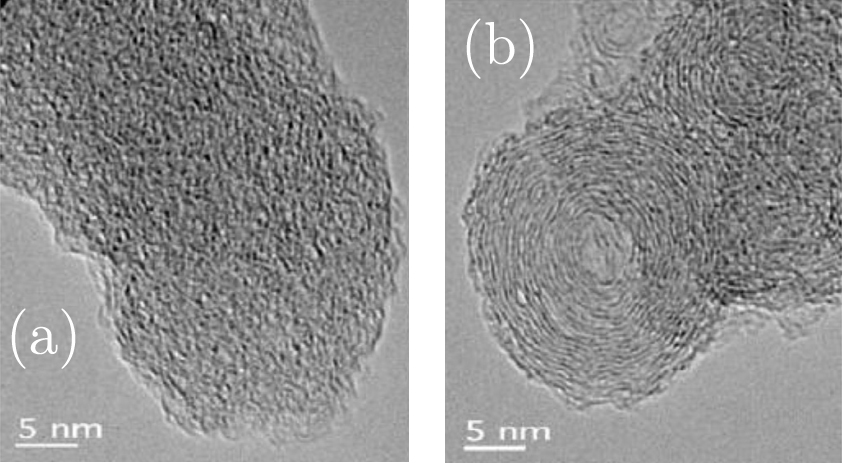
\includegraphics[height=60mm, ]{Figures/Introduction/soot_maturity.jpg}
	\caption[The HRTEM image of (a) a nascent soot primary particle juxtaposed with that of (b) a mature soot primary particle]{The HRTEM image of (a) a nascent soot primary particle with disordered internal nanostructure juxtaposed with that of (b) a mature soot primary particle with well-organized cluster near the shell sampled from soot generated by pyrolysis of ethanol at 1250 and 1650, respectively. Reprinted from Ref.\citep{vander2004soot}}
	\label{fig:sootmaturity}
\end{figure}


However, the effects of soot composition, and morphology on its refractive index, and absorption function are not fully understood yet. E(m) of soot at $\lambda=$1064 nm measured by two-color LII measurements increases from 0.193 to 0.349, and 0.226 to 0.340 for ethylene premixed flames with equivalence ratio of $\phi$=2.1 and $\phi$=2.3, respectively when height above burner (HAB) changes from 8 to 14 mm~\citep{olofsson2015evolution}. During acetylene pyrolysis in a shock tube, E(m) of soot particles increases from 0.05 to 0.25 as their primary particle diameter, $d_p$, grows to 20 nm within 1.6 ms~\citep{eremin2011size}. Using m and E(m) of mature spherical soot~\citep{dalzell1969optical} at different HABs neglecting the impact of soot morphology and composition on m~\citep{zerbs2009influence} can overestimate soot volume fraction by 100\%~\citep{kelesidis2021determination}. So, accurate estimation of the evolving optical properties of soot is essential to close the carbon mass balance in the measurements~\citep{kelesidis2021determination}, and analyze reaction kinetics for soot inception~\citep{kholghy2018reactive} surface growth~\citep{appel2000kinetic} and oxidation~\citep{puduppakkam2014soot} that are essential for development and validation of aerosol dynamics models coupled with chemistry to predict soot formation.


The dependence of soot m on its morphology and composition can be quantified by soot optical band gap, $\mathrm{E_g}$~\citep{bond2006light}. The optical band gap concept was originally proposed by \citet{tauc1966optical} for semi-conductors and later developed for amorphous carbon~\citep{robertson1987electronic}, and it can be used to describe the crystalline character of PAH clusters in soot~\citep{robertson1987electronic}. Incipient flame-made soot with diameters less than 20 nm exhibit quantum dot behavior~\citep{liu2019flame} with 0.7$<$$\mathrm{E_g}$$<$2 eV that is larger than $\mathrm{E_g}$ of graphitized soot, 0.12 eV~\citep{liu2019flame}. Optical band gap of organic carbon coated on soot remains nearly constant ($\sim$1.8-1.9 eV) over soot evolution~\citep{le2019soot}. In contrast, \citet{russo2020optical} measured soot optical band gap using ex-situ and in-situ methods and showed that $\mathrm{E_g}$ drops from 0.7 eV at HAB= 8 mm to 0.2 eV at HAB=14 mm in an ethylene premixed flame with $\phi$=2.3 as particles grow and become more mature by carbonization. \citet{kelesidis2019soot} correlated the evolving refractive index of soot with its $\mathrm{E_g}$ obtained from quantum confinement theory (QCT)~\citep{liu2019flame} for wavelengths of $\lambda$= 532 and 1064 nm~\citep{kelesidis2019soot} by linear interpolations between that of nascent and mature soot. The proposed relations were then used with soot morphologies obtained from Discrete Element Modeling (DEM) simulations to obtain the evolving Mass Absorption Cross-section (MAC), E(m), and the absorption function ratio of soot (E($\lambda$=532nm)/ E($\lambda$=1024nm)) and compared with measurements~\citep{bejaoui2015measurements, michelsen2010wavelength, cleon2011laser}. Employing the relation in laser diagnostics to reprocess light extinction measurement data resulted in accurate prediction of $f_v$ in moderate ($\phi$=2.34)~\citep{kelesidis2021determination} and rich ($\phi>$3) ethylene premixed flames~\citep{mei2021formation}, and fv along the centerline of a coflow ethylene diffusion flame~\citep{kelesidis2022santoro} which is necessary to close the carbon mass balance in soot generating processes. 

\subsection{Oxidation}
Soot oxidation is described as the removal of soot mass by reaction of molecular oxygen ($\mathrm{O_2}$), oxygen radical (O), and hydroxyl radical (OH) from soot surface. Because of its heterogeneous reaction kinetics and mechanisms, oxidation is expected to be sensitive to surface structure and composition. So, oxidation mechanisms depend on soot maturity and temperature-time history. In near stoichiometric and fuel-rich conditions, the contribution of OH radical to soot oxidation is predominant~\citep{neoh1981soot} compared to that of O radicals~\citep{lighty2009soot}. \citet{fenimore1967oxidation} investigated soot oxidation rate for low oxygen
partial pressures and temperatures from 1530 to 1890 K, highlighted the importance of OH as a major oxidation agent, and attributed the faster rates
compared to those predicted by \citet{lee1962rate}, to OH oxidation. One approach for describing OH oxidation is by a introducing collision efficiency representing the fraction of collisions of OH with soot particles that resulted in the removal of a carbon atom~\citep{neoh1981soot}. Scanning Mobility Particle Sizer (SMPS) with a two-stage burner also
showed a collision efficiency of 0.13~\citep{bartok1991fossil}.

The empirical relation of Nagle and Strickland-Constable (NSC)~\citep{nagle1962oxidation} originally developed for oxidation of pyrolytic graphite have been widely used to describe soot oxidation by $\mathrm{O_2}$. It describes $\mathrm{O_2}$ oxidation rates based on partial pressure of  $\mathrm{O_2}$ and the fraction of reactive edge sites to less reactive basal planes using the graphite analogy for soot. The dominance of edge sites in typical combustion conditions accounts for the relatively small reactivity of soot and basal planes become reactive at high temperature ($>$2500 K)~\citep{lighty2009soot}. $\mathrm{O_2}$ oxidation kinetics was also described with a power-law kinetics \cite{lee1962rate}, and shown to be first order in oxygen concentration~\citep{neeft1997kinetics}. Alternatively, soot oxidation can be explained based on chemical similarity using HACA mechanism assuming that active site are attacked by $\mathrm{O_2}$ and OH leading to loss of carbon and release of CO.

A different oxidation regime has been identified for soot at low temperatures (T$<$1000 K) where $\mathrm{O_2}$ diffuses and reacts with bulk soot accounting for most of soot mass consumption~\citep{ma2013soot}.  Internal oxidation compacts the pore network of soot resulting in hollow CB~\citep{kelesidis2022porosity}, diesel~\cite{ishiguro1991microstructural} and biodiesel~\citep{song2006examination} soot particles and increases their SSA up to a factor of four~\cite{ishiguro1991microstructural}. Oxidation can cause fragmentation of soot particles affecting their morphology. The increase in number concentration and the change of soot morphology in lean premixed flames~\citep{xu1997soot} and in the oxidation region of diffusion flames~\citep{puri1993aerosol} was attributed to fragmentation. Such a change in agglomerate morphology has not been observed in fuel-rich conditions, so fragmentation was linked to $\mathrm{O_2}$ oxidation.



%\begin{figure}[!htbp]
%	\centering
%	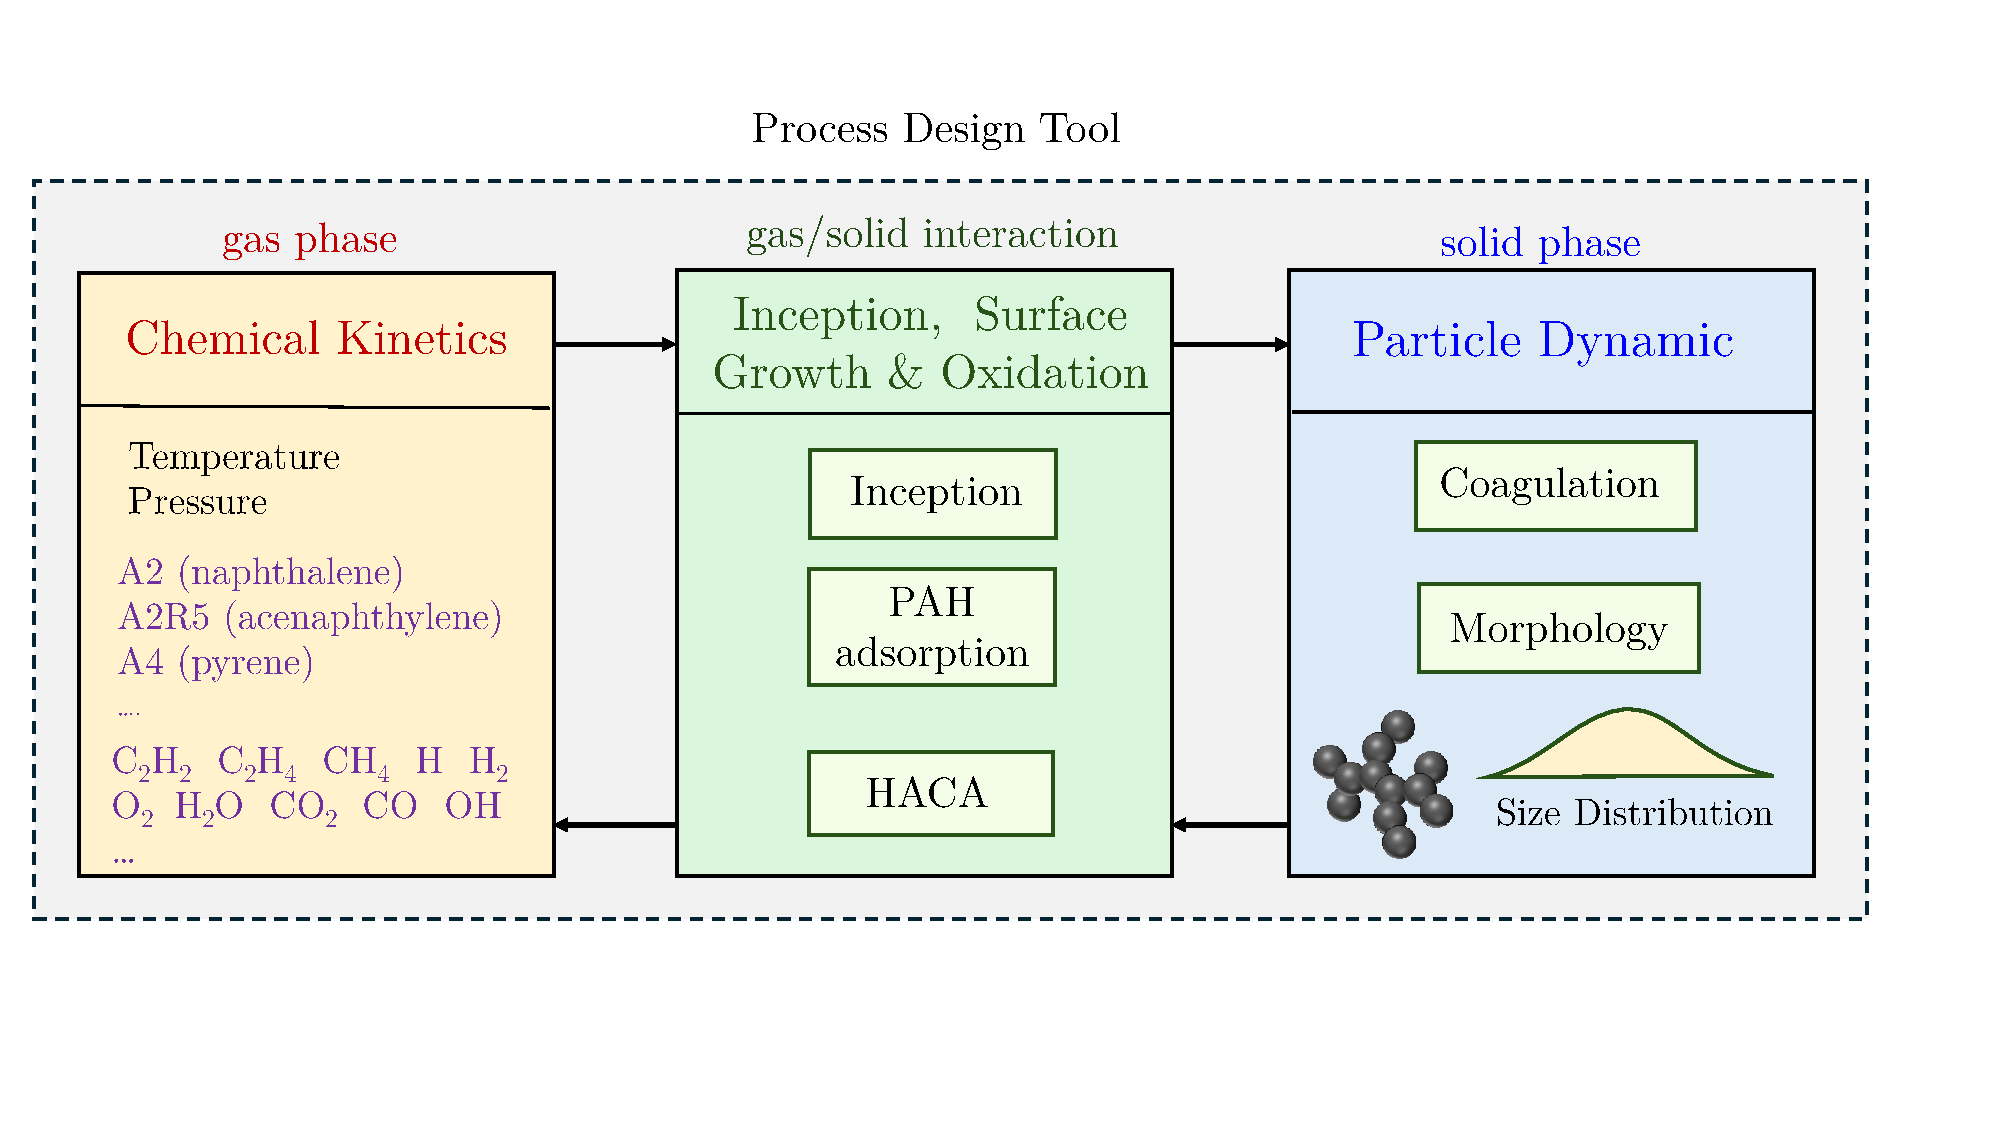
\includegraphics[height=60mm, ]{Figures/Introduction/tooldesign.pdf}
%	\caption{The conceptual structure of developed process design tool that account for gas mixture properties, and soot chemistry involving inception, surface growth and oxidation as well as its coagulation leading to the fractal-like morphology of soot particles}
%	\label{fig:tooldesign}
%\end{figure}

\section{Research objectives}

This research aims to develop an integrated computational package that extends the chemical kinetic functionality of Cantera~\citep{cantera} to predict the yield, morphology, and composition of soot formed during hydrocarbon pyrolysis and combustion. A theoretical framework is established based on zero-dimensional reactor models with simplifying assumptions that reduce the complexity of fluid dynamics and heat transfer in gas-particle systems (Section~\ref{sec:assumptions}), while emphasizing gas-phase chemical kinetics, gas-to-soot conversion, and particle dynamics. Within this framework, the transport equations for gas species and tracked soot properties were uniquely derived and implemented as part of this research (Section~\ref{sec:reactors}). In addition, governing equations for soot inception (Section~\ref{sec:pahgrowmodel}), surface growth and oxidation (Section~\ref{sec:surfreacmodel}), and coagulation (Section~\ref{sec:particledynamics}) from the literature are described in detail. A new inception model based on E-Bridge formation~\citep{frenklach2020mechanism}, referred to as E-Bridge Modified, was proposed and further refined for consistency with the Omnisoot implementation (Section~\ref{sec:ebrimod}). A rigorous multi-step validation procedure was followed to ensure the reliability of the model predictions (Chapter~\ref{sec:particledynamics}).

The ultimate goal of this work is to provide a process design and optimization tool for carbon black synthesis that offers insight into the influence of process parameters, such as pressure, temperature time history, and residence time, on carbon black structure, including agglomerate size and specific surface area, as key performance indicators~\citep{murphy2001additives}. Such a tool also enables systematic investigation of the effects of additives on pyrolysis chemistry, inception flux, and surface growth rates, which ultimately determine carbon black properties. Two notable examples are hydrogen, which has a well-established inhibitory effect on PAH and soot formation~\citep{eremin2012experimental}, and toluene, which promotes soot inception~\citep{harris1984soot}. Omnisoot simulations were employed to elucidate the impact of hydrogen addition on soot yield, morphology, and maturity during shock-tube pyrolysis of methane. The results and analysis of this study, the first paper in the list of secondary publications, are not included here to prioritize the main contributions of the author. Ongoing work further examines the combined effects of hydrogen and toluene on methane pyrolysis.

Model versatility is a central development principle of Omnisoot. The package allows any detailed kinetic mechanism in Cantera format to be coupled with particle dynamics through inception, surface growth, and oxidation models, thereby enabling the assessment of uncertainties arising from gas-phase chemistry due to variability in reaction pathways and rate constants. Leveraging this flexible structure, the fundamental differences among the implemented inception models were analyzed in terms of their temperature dependence. Predictions of soot yield, morphology, and particle size distribution obtained using these inception models were compared against benchmark measurements from methane and ethylene pyrolysis and combustion (Section~\ref{sec:paper1_fanalysis_inception_models}).

The performance of several kinetic mechanisms was evaluated for predicting key intermediate species during shock-tube pyrolysis of methane at high fuel loadings. Simulation results were used to explain differences among mechanisms in terms of dominant pathways that transfer carbon from methane to larger intermediates, such as ethylene, acetylene, and propargyl. The mechanism that best reproduces the measured species profiles was selected for detailed soot analysis. These investigations indicate that the E-Bridge Modified inception model captures both the temperature dependence and time history of soot volume fraction in good agreement with light extinction measurements (Section~\ref{sec:paper2_high_fuel_loadings}).

The same combination of kinetic mechanism and inception model was subsequently applied to identify distinct stages of soot formation. The proposed coupled model successfully predicts primary particle diameters in close agreement with TEM measurements, while the sources of observed model-data discrepancies were discussed in terms of precursor chemistry and potential late-stage processes not represented in Omnisoot due to theoretical limitations. A carbonization model was employed to describe the evolution of soot composition and the associated reduction in active sites for surface growth. A strong correspondence was demonstrated between the modeled soot hydrogen-to-carbon ratio and the maturity index inferred from extinction ratios at two wavelengths (Section~\ref{sec:paper3_stages_soot_formations}).

Finally, it is noted that the oxidation model implemented in Omnisoot is functional and has been applied in limited cases, but it has not been thoroughly validated against benchmark data due to the scarcity of measurements relevant to zero-dimensional reactors. Furthermore, the scope of this work is primarily focused on soot formation in the absence of oxidizing agents such as O$_2$ and OH.

%% brainstorming for research objectives
% Developing a integrated platform that extends the chemical kinetic functionality of Cantera to predict yield, morphology and composition of soot formed during pyrolysis and combustion of hydrocarbons. A theoretical framework is established based on zero-dimentional reactors with simplyfying assumptions to reduce the complexity of fluid dynamics and heat transfer aspects of the problem in favor of chemical kinetics, gas-to-soot conversion, and particle dynamics. The transport equations for gas species and tracked soot properties are derived specifically for this research and implemented in the package. Additionally, the governaning equations for inception, surface growth, oxidation and coagulation from the literature explained in detail. A new inception model based on E-Bridge formation, E-Bridge Modified, was proposed and extended with certain modifications for consistency with Omnisoot implementation. A rigoruos multi-step validation procedure was follow to ensure the reliability of model results.

%This research is aimed at developing an a integrated computational package that extends the chemical kinetic functionality of Cantera~\citep{cantera} to predict yield, morphology and composition of soot formed during pyrolysis and combustion of hydrocarbons. A theoretical framework was established based on zero-dimensional reactor models with simplifying assumptions to reduce the complexity of fluid dynamics and heat transfer aspects of gas-particle system  in favor of gas chemical kinetics, gas-to-soot conversion, and particle dynamics. The transport equations for gas species and tracked soot properties are derived uniquely for this research and implemented in the package. Additionally, the governing equations for soot inception, surface growth, oxidation and coagulation from the literature are explained in detail. A new inception model based on E-Bridge formation, E-Bridge Modified, was proposed and extended with certain modifications for consistency with Omnisoot implementation. A rigorous multi-step validation procedure was follow to ensure the reliability of model results.

%The ultimate goal is to have a process design and optimization tool for CB synthesis to provide insight into the effect of process parameter, such as pressure, temperature time history, and residence time, on CB structure (agglomerate size) and SSA, as key performance indicators of CB~\citep{murphy2001additives}. Such a tool also provides insight into the influence of additives on pyrolysis chemistry, inception flux, and surface growth rate that determine final CB properties. Two prominent examples are hydrogen with widely known inhibitory effect on PAH and soot formation~\citep{eremin2012experimental}, and toluene, promoting soot inception~\citep{harris1984soot}. Omnisoot simulations were used to elucidate the impact of hydrogen addition on soot yield, morphology, and maturity formed by shock-tube pyrolysis of methane. The results and analysis (listed as the fourth publication in ***) are not included here to prioritize the main contributions of the author instead. In an ongoing research, the compounded effect of hydrogen and toluene on methane pyrolysis is investigated.

%Model versatility is a main development principle. Omnisoot allows any detailed kinetic mechanism in Cantera format to be interfaced with particle dynamics through inception, surface growth, and oxidation models, which enables highlighting the uncertainties that originates from gas chemistry due to variability in rate constants and pathways. Capitalizing on the flexible structure, the fundamental differences between the implemented inception model are explained in terms of their temperature dependence. Soot yield, morphology, particle size distribution predicted using the inception models are compared with benchmark measurement in pyrolysis and combustion of methane and ethylene.

%The performance of several kinetic mechanisms are compared for prediction of key intermediates during shock-tube pyrolysis of methane at high fuel loadings. The simulation results are used to explained the difference between mechanisms in terms of major pathways that transfer carbon from methane to larger intermediates such ethylene, acetylene and propargyl. The mechanism with the results closer to species measurements is chosen for detail soot analysis. The investigations indicated that E-Bridge Modified model captures the temperature trend and time-history of soot volume fraction in good agreement with light extinction data.

%The same combination of kinetic mechanism and inception model is used to identify stages of soot formation. The proposed combined model successfully predicts primary particle diameter in close agreement with TEM measurements, and the sources of observed model-data deviations are explained in terms of precursor chemistry followed potential scenarios not accounted for in Omnisoot due to theoretical limitations. A carbonization model is used to describe evolution of soot composition that limits active sites for surface growth, and strong correspondence is highlighted between soot hydrogen-to-carbon ratio with maturity index inferred from extinction ratio at two wavelengths.

%Note that, the oxidation model implemented in Omnisoot is functional and used in limited cases, but it has not been thoroughly compared against benchmark data due to scarcity of measurements relevant to 0D reactors. Furthermore, the scope of this work is mainly focused on soot formation in the absence of oxidizing agents such as O$_2$ and OH.
 



% 
\section{Code availability}

Omnisoot is published as a standard Python package and is publicly accessible through PyPi\footnote{\href{https://pypi.org/project/omnisoot/}{https://pypi.org/project/omnisoot/}}. The programming interface provides an easy-to-use workflow that allows users to load reaction mechanisms via Cantera, select reactor configurations, and specify the desired soot sub-models. Multiple example scripts are provided in the public GitHub repository\footnote{\href{https://github.com/mohammadadib-cu/omnisoot-cv/tree/main/examples}{https://github.com/mohammadadib-cu/omnisoot-cv/tree/main/examples}} of Omnisoot to demonstrate typical workflows and to enable developing custom simulations for various applications. In addition, the validation scripts used in this work are available in the same repository\footnote{\href{https://github.com/mohammadadib-cu/omnisoot-cv/tree/main/validations}{https://github.com/mohammadadib-cu/omnisoot-cv/tree/main/validations}} for transparency and community feedback.


